\subsection{Generating Noisy Queries}
\label{sec:making-noise}
While previous work has studied the impact of minor variations to queries, such as typos and misspellings, query noise is much more diverse. Seeking to expand this understanding, we explore the impact of query alterations that evaluate surface, syntactic, and semantic alterations. To apply noise to a query, we either edit a query to introduce a specific type of noise or rewrite the query to simulate similarly worded intents. Each query that is altered has a notion of its anchor, either a character, word or a group of words, which is selected where noise is applied. To achieve this for each query, a character or word index is randomly selected. Then, noise is applied to the left, right, or at the noising index (replacing the existing index) with equal probability. Example alterations are in table \ref{tab:query-noise}. \\
To study the impact of surface-level alterations, we introduce noise in queries by simulating misspellings and typos by swapping, eliminating, or shuffling characters in a query. To understand how models respond to typos or character omissions, we delete a character (DC), inject a random character (RCS), or simulate a keyboard-based typo by injecting a character close to its neighbor on a keyboard (KCS). We swap the indexed word with another word in the query to understand how systems may work when faced with natural shifts in keyword queries. \\
To study syntactic alterations, we introduce noise that alters the syntax of the query introducing lemmas, stems, synonyms, and determiners using tools from the NLTK toolkit \cite{bird2009natural}. Synonyms are introduced using NLTK's interface with WordNet \cite{Fellbaum2000WordNetA}, and exact synonyms for a single word are introduced.  Determiners, affixes that occur with nouns and commonly are not discriminative for search, are introduced similarly to typos to the left or right of noun phrases. Lemma's return words to their canonical root while stemming reduced word inflection using the Porter-stemmer. We select up to five words per query to attempt stemming/lemmatization, but many queries do not have any words which can be stemmed or lemmatized versions and, as a result, are un-noised. \\
Exploring semantically similar queries, we leverage paraphrasing, back-translation, and synonyms. To paraphrase, we rewrite queries using a T5 \cite{Raffel2020ExploringTL} sequence-to-sequence model, which has been fine-tuned on the PAWS \cite{Zhang2019PAWSPA} dataset. For back-translation, we use OpenNMT's \cite{klein-etal-2017-opennmt} to translate queries from English to another language and then back to English after exploring performance using German, French, Italian, and Spanish to find the German to have the best quality and use only those. It is worth noting that these semantic noising methods are the most likely to alter the true query intent, as seen by the 'hallucinations' in table \ref{tab:query-noise} paraphrase alteration. \\
Using the aforementioned noising approaches, we noise the queries on the MSMARCO \cite{Campos2016MSMA} \footnote{https://huggingface.co/datasets/spacemanidol/msmarco-passage-query-variation} \footnote{https://huggingface.co/datasets/spacemanidol/rewrite-noisy-queries}, Natural Questions \footnote{https://huggingface.co/datasets/spacemanidol/wikipedia-nq-query-variation} \footnote{https://huggingface.co/datasets/spacemanidol/nq-noising} \cite{Kwiatkowski2019NaturalQA}, and the Trivia QA \cite{Joshi2017TriviaQAAL} \footnote{https://huggingface.co/datasets/spacemanidol/wikipedia-trivia-query-variation} Passage Ranking datasets. \\
\subsection{Baseline Performance}
\begin{figure}[!htb]
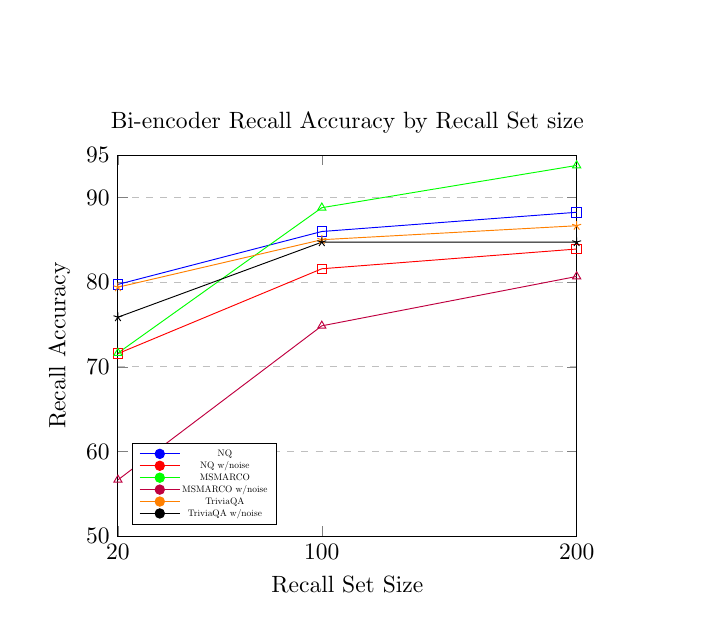
\begin{tikzpicture}
\scalebox{0.85}{
\begin{axis}[
    title={Bi-encoder Recall Accuracy by Recall Set size},
    xlabel={Recall Set Size},
    ylabel={Recall Accuracy},
    xmin=20, xmax=200,
    ymin=50 , ymax=95,
    xtick={20, 100, 200},
    ytick={50, 60, 70, 80, 90, 95},
    legend pos=south west,
    ymajorgrids=true,
    grid style=dashed,
    legend style={nodes={scale=0.4, transform shape}}, 
    legend image post style={mark=*}
]
\addplot[
    color=blue,
    mark=square,
    ]
    coordinates {
    (20, 79.73) (100, 85.98) (200, 88.25)
    };
\addplot[
    color=red,
    mark=square,
    ]
    coordinates {
    (20, 71.56) (100,81.58) (200, 83.91)
    };
\addplot[
    color=green,
    mark=triangle,
    ]
    coordinates {
    (20, 71.63) (100, 88.79) (200, 93.78)
    };
    
\addplot[
    color=purple,
    mark=triangle,
    ]
    coordinates {
    (20, 56.65) (100, 74.84) (200, 80.67)
    };
\addplot[
    color=orange,
    mark=star,
    ]
    coordinates {
    (20, 79.40) (100,85.01) (200, 86.66)
    };
\addplot[
    color=black,
    mark=star,
    ]
    coordinates {
    (20, 75.86) (100, 84.72) (200, 84.72)
    };
\legend{NQ, NQ w/noise, MSMARCO, MSMARCO w/noise, TriviaQA, TriviaQA w/noise}
 \end{axis}}
\end{tikzpicture}
    \centering
    \caption{Bi-encoder recall accuracy on noisy and non-noisy queries with variations of recall set size and datasets. }
    \label{fig:baseline-impact-query-noise}
\end{figure}
In production workloads, bi-encoders are most commonly used for early retrieval, where the sets they produce are then reranked using a cross-encoder. Given cross-encoder are more robust to typos \cite{Sidiropoulos2022AnalysingTR}, our work focuses exclusively on evaluating the impact of noise on the retrieval accuracy of bi-encoders. \\
To do so, we train  a series of task-specific bi-encoders leveraging the open-source bi-encoder-focused library Tevatron \cite{Gao2022TevatronAE} with task-specific training parameters found in \ref{tab:capot-bi-encoder-hy} on the widely used and studied MSMARCO \cite{Campos2016MSMA}, Natural Questions (NQ) \cite{Kwiatkowski2019NaturalQA} and TriviaQA \cite{Joshi2017TriviaQAAL} passage retrieval datasets. \\
For contextual representations, each encoder uses  a pre-trained BERT \cite{Devlin2019BERTPO} model for its initialization, and we use separate models for the query and document models. Representations are taken from the unaltered 768-dimension vectors based on the last hidden representation of the CLS token. \\
For each dataset, we train each model using 5 different random seeds with fixed optimal hyperparameters, generate seed and task-specific indexes and evaluate the retrieval impact of queries with noise and unaltered routes. We evaluate the impact on retrieval by measuring the impact on retrieval accuracy at $k$ with a $k={20,100,200}$.  \\
As shown in figure \ref{fig:baseline-impact-query-noise} on the impact of averaged noise, our experimental results align with prior research. There is a wide variation of impact as the long, trivia-inspired queries of Trivia QA see minor losses in accuracy compared to the real-world web search queries of MSMARCO, up to 12\% the impact. Besides the impact of query type, we also notice the large role recall set size plays on the relative degradation in retrieval accuracy. Across tasks and datasets, increasing the recall set from 20 to 200 decreases the impact on accuracy by about 50\%. \\ 
Focusing on the impacts of individual types of noise shown in \ref{sec:full-noise-impact}, we see that queries with surface alteration, such as typos, see the largest loss. Despite featuring real-world search engine queries with noise, on MSMARCO, there is nearly a 30\% loss in retrieval accuracy for queries with typos, dropping from 71\% to 41\%. On all datasets, queries with character-level alterations see a 50\% average higher loss in accuracy than other alterations. This large gap can be attributed to the vocabulary construction method of BERT and BERT-like models, where a minor alteration to a single character can produce large variations in tokenization.\\
In the absence of model optimization, data augmentation, or post-training optimization, the clearest way to make dense retrieval robust to noise is to expand the recall set and allow cross-encoders to re-rank the expanded results.\\